\section{Quadrature}

The central building block for evaluating inner products is the calculation of
integrals between wavepackets.
This is done numerically with a quadrature rule, of which there are many
different kinds.


\subsection{Gauss-Hermite Quadrature}
\label{subsec:ghquad}

The basic integration algorithm used in this project is the one-dimensional
Gauss-Hermite quadrature.
Like related rules, this method works by evaluating the integrand function at a
defined set of nodes $\gamma_i$, the values of which are summed up with specific
weights $\omega_i$:

\begin{equation}
  \label{eq:gaussquad}
  \int_{-\infty}^{\infty} g(x) \, dx \approx \sum_{i=1}^{n} f(\gamma_i) \omega_i
\end{equation}

In its basic form, the Gauss-Hermite rule works on special integrals of the
following form:

\begin{equation}
  \int_{-\infty}^{\infty} e^{-x^2} f(x) \, dx
\end{equation}

However, as we require the quadrature to work on general functions,
transformations are done to the usual weights and nodes which is described in
\cite{B_master_thesis}.
The result is a rule in the form of \eqref{eq:gaussquad}.
Figure~\ref{fig:ghexample} shows an example of the node distribution of a
Gauss-Hermite rule.

\begin{figure}
  \center
  % GNUPLOT: LaTeX picture with Postscript
\begingroup
  \makeatletter
  \providecommand\color[2][]{%
    \GenericError{(gnuplot) \space\space\space\@spaces}{%
      Package color not loaded in conjunction with
      terminal option `colourtext'%
    }{See the gnuplot documentation for explanation.%
    }{Either use 'blacktext' in gnuplot or load the package
      color.sty in LaTeX.}%
    \renewcommand\color[2][]{}%
  }%
  \providecommand\includegraphics[2][]{%
    \GenericError{(gnuplot) \space\space\space\@spaces}{%
      Package graphicx or graphics not loaded%
    }{See the gnuplot documentation for explanation.%
    }{The gnuplot epslatex terminal needs graphicx.sty or graphics.sty.}%
    \renewcommand\includegraphics[2][]{}%
  }%
  \providecommand\rotatebox[2]{#2}%
  \@ifundefined{ifGPcolor}{%
    \newif\ifGPcolor
    \GPcolortrue
  }{}%
  \@ifundefined{ifGPblacktext}{%
    \newif\ifGPblacktext
    \GPblacktexttrue
  }{}%
  % define a \g@addto@macro without @ in the name:
  \let\gplgaddtomacro\g@addto@macro
  % define empty templates for all commands taking text:
  \gdef\gplbacktext{}%
  \gdef\gplfronttext{}%
  \makeatother
  \ifGPblacktext
    % no textcolor at all
    \def\colorrgb#1{}%
    \def\colorgray#1{}%
  \else
    % gray or color?
    \ifGPcolor
      \def\colorrgb#1{\color[rgb]{#1}}%
      \def\colorgray#1{\color[gray]{#1}}%
      \expandafter\def\csname LTw\endcsname{\color{white}}%
      \expandafter\def\csname LTb\endcsname{\color{black}}%
      \expandafter\def\csname LTa\endcsname{\color{black}}%
      \expandafter\def\csname LT0\endcsname{\color[rgb]{1,0,0}}%
      \expandafter\def\csname LT1\endcsname{\color[rgb]{0,1,0}}%
      \expandafter\def\csname LT2\endcsname{\color[rgb]{0,0,1}}%
      \expandafter\def\csname LT3\endcsname{\color[rgb]{1,0,1}}%
      \expandafter\def\csname LT4\endcsname{\color[rgb]{0,1,1}}%
      \expandafter\def\csname LT5\endcsname{\color[rgb]{1,1,0}}%
      \expandafter\def\csname LT6\endcsname{\color[rgb]{0,0,0}}%
      \expandafter\def\csname LT7\endcsname{\color[rgb]{1,0.3,0}}%
      \expandafter\def\csname LT8\endcsname{\color[rgb]{0.5,0.5,0.5}}%
    \else
      % gray
      \def\colorrgb#1{\color{black}}%
      \def\colorgray#1{\color[gray]{#1}}%
      \expandafter\def\csname LTw\endcsname{\color{white}}%
      \expandafter\def\csname LTb\endcsname{\color{black}}%
      \expandafter\def\csname LTa\endcsname{\color{black}}%
      \expandafter\def\csname LT0\endcsname{\color{black}}%
      \expandafter\def\csname LT1\endcsname{\color{black}}%
      \expandafter\def\csname LT2\endcsname{\color{black}}%
      \expandafter\def\csname LT3\endcsname{\color{black}}%
      \expandafter\def\csname LT4\endcsname{\color{black}}%
      \expandafter\def\csname LT5\endcsname{\color{black}}%
      \expandafter\def\csname LT6\endcsname{\color{black}}%
      \expandafter\def\csname LT7\endcsname{\color{black}}%
      \expandafter\def\csname LT8\endcsname{\color{black}}%
    \fi
  \fi
  \setlength{\unitlength}{0.0500bp}%
  \begin{picture}(7200.00,4320.00)%
    \gplgaddtomacro\gplbacktext{%
      \csname LTb\endcsname%
      \put(946,704){\makebox(0,0)[r]{\strut{} 0}}%
      \csname LTb\endcsname%
      \put(946,1123){\makebox(0,0)[r]{\strut{} 0.1}}%
      \csname LTb\endcsname%
      \put(946,1542){\makebox(0,0)[r]{\strut{} 0.2}}%
      \csname LTb\endcsname%
      \put(946,1961){\makebox(0,0)[r]{\strut{} 0.3}}%
      \csname LTb\endcsname%
      \put(946,2380){\makebox(0,0)[r]{\strut{} 0.4}}%
      \csname LTb\endcsname%
      \put(946,2798){\makebox(0,0)[r]{\strut{} 0.5}}%
      \csname LTb\endcsname%
      \put(946,3217){\makebox(0,0)[r]{\strut{} 0.6}}%
      \csname LTb\endcsname%
      \put(946,3636){\makebox(0,0)[r]{\strut{} 0.7}}%
      \csname LTb\endcsname%
      \put(946,4055){\makebox(0,0)[r]{\strut{} 0.8}}%
      \csname LTb\endcsname%
      \put(1078,484){\makebox(0,0){\strut{}-10}}%
      \csname LTb\endcsname%
      \put(1651,484){\makebox(0,0){\strut{}-8}}%
      \csname LTb\endcsname%
      \put(2223,484){\makebox(0,0){\strut{}-6}}%
      \csname LTb\endcsname%
      \put(2796,484){\makebox(0,0){\strut{}-4}}%
      \csname LTb\endcsname%
      \put(3368,484){\makebox(0,0){\strut{}-2}}%
      \csname LTb\endcsname%
      \put(3941,484){\makebox(0,0){\strut{} 0}}%
      \csname LTb\endcsname%
      \put(4513,484){\makebox(0,0){\strut{} 2}}%
      \csname LTb\endcsname%
      \put(5086,484){\makebox(0,0){\strut{} 4}}%
      \csname LTb\endcsname%
      \put(5658,484){\makebox(0,0){\strut{} 6}}%
      \csname LTb\endcsname%
      \put(6231,484){\makebox(0,0){\strut{} 8}}%
      \csname LTb\endcsname%
      \put(6803,484){\makebox(0,0){\strut{} 10}}%
      \put(176,2379){\makebox(0,0){\strut{}$\omega_i$}}%
      \put(3940,154){\makebox(0,0){\strut{}$\gamma_i$}}%
    }%
    \gplgaddtomacro\gplfronttext{%
    }%
    \gplbacktext
    \put(0,0){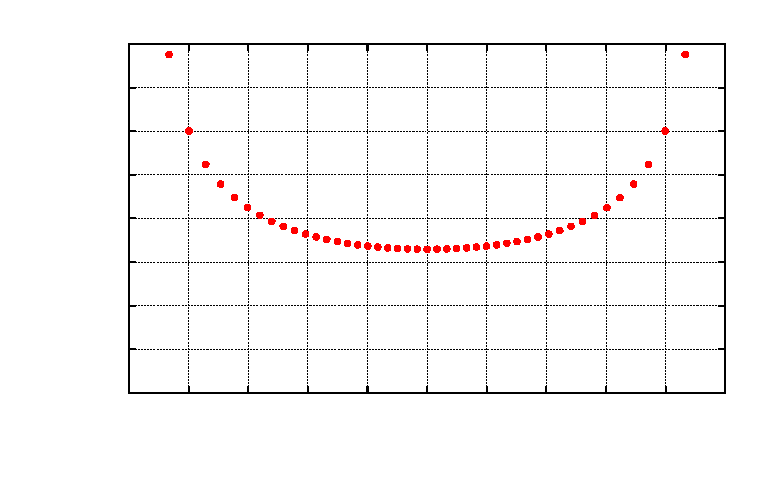
\includegraphics{gh-rule}}%
    \gplfronttext
  \end{picture}%
\endgroup

  \caption{45-point Gauss-Hermite nodes and weights}
  \label{fig:ghexample}
\end{figure}

In the implementation of this rule, an auxiliary Python script was made to
automatically generate C++-code with hardcoded tables of nodes and weights for
different orders.


\subsection{Tensor-Product Quadrature}
\label{subsec:tpquad}

The wavepackets that are processed by WaveBlocks are generally multi-dimensional.
To handle this, tensor products of $D$ one-dimensional quadrature rules can be
built up.

Denoting the $i$-th node-weight-pair of the $d$-th scalar quadrature rule
$(\gamma_i^d,\ \omega_i^d)$, the resulting pair at the multi-index $j = (j_1,
\ldots, j_d)$ for the resulting tensor quadrature rule is:

\begin{equation}
  (\gamma_j,\ \omega_j) = \left(
    \begin{pmatrix} \gamma_{j_1}^1 \\ \vdots \\ \gamma_{j_d}^d \end{pmatrix},
    \ \prod_{d=1}^D \omega_{j_d}^d
  \right)
\end{equation}

A two-dimensional quadrature rule is shown in figure~\ref{fig:tpexample}.

\begin{figure}
  \center
  % GNUPLOT: LaTeX picture with Postscript
\begingroup
  \makeatletter
  \providecommand\color[2][]{%
    \GenericError{(gnuplot) \space\space\space\@spaces}{%
      Package color not loaded in conjunction with
      terminal option `colourtext'%
    }{See the gnuplot documentation for explanation.%
    }{Either use 'blacktext' in gnuplot or load the package
      color.sty in LaTeX.}%
    \renewcommand\color[2][]{}%
  }%
  \providecommand\includegraphics[2][]{%
    \GenericError{(gnuplot) \space\space\space\@spaces}{%
      Package graphicx or graphics not loaded%
    }{See the gnuplot documentation for explanation.%
    }{The gnuplot epslatex terminal needs graphicx.sty or graphics.sty.}%
    \renewcommand\includegraphics[2][]{}%
  }%
  \providecommand\rotatebox[2]{#2}%
  \@ifundefined{ifGPcolor}{%
    \newif\ifGPcolor
    \GPcolortrue
  }{}%
  \@ifundefined{ifGPblacktext}{%
    \newif\ifGPblacktext
    \GPblacktexttrue
  }{}%
  % define a \g@addto@macro without @ in the name:
  \let\gplgaddtomacro\g@addto@macro
  % define empty templates for all commands taking text:
  \gdef\gplbacktext{}%
  \gdef\gplfronttext{}%
  \makeatother
  \ifGPblacktext
    % no textcolor at all
    \def\colorrgb#1{}%
    \def\colorgray#1{}%
  \else
    % gray or color?
    \ifGPcolor
      \def\colorrgb#1{\color[rgb]{#1}}%
      \def\colorgray#1{\color[gray]{#1}}%
      \expandafter\def\csname LTw\endcsname{\color{white}}%
      \expandafter\def\csname LTb\endcsname{\color{black}}%
      \expandafter\def\csname LTa\endcsname{\color{black}}%
      \expandafter\def\csname LT0\endcsname{\color[rgb]{1,0,0}}%
      \expandafter\def\csname LT1\endcsname{\color[rgb]{0,1,0}}%
      \expandafter\def\csname LT2\endcsname{\color[rgb]{0,0,1}}%
      \expandafter\def\csname LT3\endcsname{\color[rgb]{1,0,1}}%
      \expandafter\def\csname LT4\endcsname{\color[rgb]{0,1,1}}%
      \expandafter\def\csname LT5\endcsname{\color[rgb]{1,1,0}}%
      \expandafter\def\csname LT6\endcsname{\color[rgb]{0,0,0}}%
      \expandafter\def\csname LT7\endcsname{\color[rgb]{1,0.3,0}}%
      \expandafter\def\csname LT8\endcsname{\color[rgb]{0.5,0.5,0.5}}%
    \else
      % gray
      \def\colorrgb#1{\color{black}}%
      \def\colorgray#1{\color[gray]{#1}}%
      \expandafter\def\csname LTw\endcsname{\color{white}}%
      \expandafter\def\csname LTb\endcsname{\color{black}}%
      \expandafter\def\csname LTa\endcsname{\color{black}}%
      \expandafter\def\csname LT0\endcsname{\color{black}}%
      \expandafter\def\csname LT1\endcsname{\color{black}}%
      \expandafter\def\csname LT2\endcsname{\color{black}}%
      \expandafter\def\csname LT3\endcsname{\color{black}}%
      \expandafter\def\csname LT4\endcsname{\color{black}}%
      \expandafter\def\csname LT5\endcsname{\color{black}}%
      \expandafter\def\csname LT6\endcsname{\color{black}}%
      \expandafter\def\csname LT7\endcsname{\color{black}}%
      \expandafter\def\csname LT8\endcsname{\color{black}}%
    \fi
  \fi
  \setlength{\unitlength}{0.0500bp}%
  \begin{picture}(7200.00,5040.00)%
    \gplgaddtomacro\gplbacktext{%
      \csname LTb\endcsname%
      \put(942,1289){\makebox(0,0){\strut{}-5}}%
      \csname LTb\endcsname%
      \put(1266,1230){\makebox(0,0){\strut{}-4}}%
      \csname LTb\endcsname%
      \put(1590,1170){\makebox(0,0){\strut{}-3}}%
      \csname LTb\endcsname%
      \put(1914,1111){\makebox(0,0){\strut{}-2}}%
      \csname LTb\endcsname%
      \put(2238,1051){\makebox(0,0){\strut{}-1}}%
      \csname LTb\endcsname%
      \put(2562,992){\makebox(0,0){\strut{} 0}}%
      \csname LTb\endcsname%
      \put(2886,933){\makebox(0,0){\strut{} 1}}%
      \csname LTb\endcsname%
      \put(3209,873){\makebox(0,0){\strut{} 2}}%
      \csname LTb\endcsname%
      \put(3533,814){\makebox(0,0){\strut{} 3}}%
      \csname LTb\endcsname%
      \put(3856,754){\makebox(0,0){\strut{} 4}}%
      \csname LTb\endcsname%
      \put(4180,695){\makebox(0,0){\strut{} 5}}%
      \csname LTb\endcsname%
      \put(4398,755){\makebox(0,0){\strut{}-8}}%
      \csname LTb\endcsname%
      \put(4632,884){\makebox(0,0){\strut{}-6}}%
      \csname LTb\endcsname%
      \put(4866,1013){\makebox(0,0){\strut{}-4}}%
      \csname LTb\endcsname%
      \put(5100,1141){\makebox(0,0){\strut{}-2}}%
      \csname LTb\endcsname%
      \put(5333,1270){\makebox(0,0){\strut{} 0}}%
      \csname LTb\endcsname%
      \put(5567,1398){\makebox(0,0){\strut{} 2}}%
      \csname LTb\endcsname%
      \put(5801,1527){\makebox(0,0){\strut{} 4}}%
      \csname LTb\endcsname%
      \put(6035,1656){\makebox(0,0){\strut{} 6}}%
      \csname LTb\endcsname%
      \put(6268,1784){\makebox(0,0){\strut{} 8}}%
      \put(920,1384){\makebox(0,0)[r]{\strut{} 0}}%
      \put(920,1613){\makebox(0,0)[r]{\strut{} 0.1}}%
      \put(920,1842){\makebox(0,0)[r]{\strut{} 0.2}}%
      \put(920,2070){\makebox(0,0)[r]{\strut{} 0.3}}%
      \put(920,2299){\makebox(0,0)[r]{\strut{} 0.4}}%
      \put(920,2527){\makebox(0,0)[r]{\strut{} 0.5}}%
      \put(920,2755){\makebox(0,0)[r]{\strut{} 0.6}}%
      \put(920,2984){\makebox(0,0)[r]{\strut{} 0.7}}%
      \put(920,3212){\makebox(0,0)[r]{\strut{} 0.8}}%
      \put(920,3441){\makebox(0,0)[r]{\strut{} 0.9}}%
      \put(188,2413){\makebox(0,0){\strut{}$\omega_i$}}%
    }%
    \gplgaddtomacro\gplfronttext{%
      \csname LTb\endcsname%
      \put(2264,677){\makebox(0,0){\strut{}$\gamma_i^1$}}%
      \put(6029,1156){\makebox(0,0){\strut{}$\gamma_i^2$}}%
      \put(188,2413){\makebox(0,0){\strut{}$\omega_i$}}%
    }%
    \gplbacktext
    \put(0,0){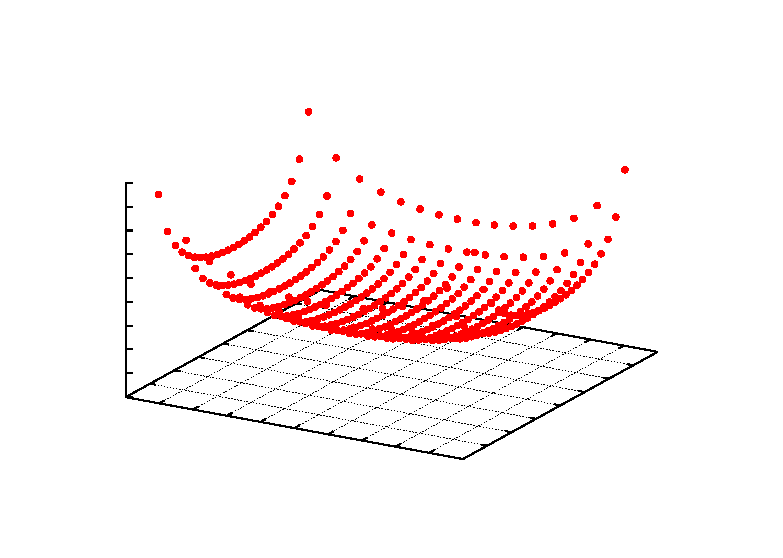
\includegraphics{tp-rule}}%
    \gplfronttext
  \end{picture}%
\endgroup

  \caption{Tensor-product built from 16- and 25-point Gauss-Hermite rules}
  \label{fig:tpexample}
\end{figure}


\subsection{Result Caching}

As the node positions and weight values are tabulated with an external script
for Gauss-Hermite Quadrature (\ref{subsec:ghquad}), the code for looking up and
returning those numbers is simple and fast.

However, in the case of Tensor-Product Quadrature (\ref{subsec:tpquad}), some
calculations must be performed to yield these values.
We wish to avoid re-calculating node and weight vectors when the same quadrature
rule is used many times, as is done in the case of wavepacket propagation over
many iterations.

For this reason, the results are only calculated once for a given Tensor-Product
rule, stored and re-used automatically on subsequent queries.
The quadrature functions have been implemented as \texttt{static} methods, with
the rule parameters given as template parameters.
Therefore, the caching is done in \texttt{static} fields.

This has the advantage that the rule only has to be calculated once in the
entire run of the program as long as the quadrature rule is the same, even if it
is invoked in different scopes, without having to pass down an object explicitly
that holds a state.
On the other hand, no clean-up can be done automatically, so a method must be
called manually to free the memory used by the cache.
